% =============================================================================
%  Paper 009 — Calibrating Human Oversight for Clinical AI Agents
%  QUOKKAGUARD paper program. House style from papers/_template (Quome logo).
% =============================================================================
\documentclass[11pt]{article}
\usepackage[utf8]{inputenc}
\usepackage[margin=1in]{geometry}
\usepackage{booktabs}
\usepackage{graphicx}
\usepackage{float}
\usepackage{afterpage}
\usepackage[section]{placeins}
\renewcommand{\topfraction}{0.9}
\renewcommand{\bottomfraction}{0.8}
\renewcommand{\textfraction}{0.08}
\renewcommand{\floatpagefraction}{0.75}
\setcounter{topnumber}{3}
\setcounter{bottomnumber}{2}
\setcounter{totalnumber}{5}
\usepackage{amsmath}
\usepackage{amssymb}
\usepackage{hyperref}
\usepackage{xcolor}
\usepackage{listings}
\definecolor{kwblue}{rgb}{0.10,0.20,0.65}
\definecolor{typepurple}{rgb}{0.50,0.15,0.55}
\definecolor{strred}{rgb}{0.62,0.12,0.12}
\definecolor{cmtgreen}{rgb}{0.20,0.45,0.20}
\lstdefinestyle{housespecyaml}{
  basicstyle=\ttfamily\footnotesize,
  backgroundcolor=\color{black!3},
  frame=single,
  framesep=5pt,
  rulecolor=\color{black!45},
  columns=fullflexible,
  breaklines=true,
  keepspaces=true,
  showstringspaces=false,
  alsoletter=_,
  commentstyle=\color{cmtgreen}\itshape,
  stringstyle=\color{strred},
  morecomment=[l]{\#},
  morestring=[b]",
  morestring=[b]',
  keywordstyle=\color{kwblue}\bfseries,
  keywords={tool_risk,allow_below,deny_above,temperature,bands,calibration,timeout},
  keywordstyle=[2]\color{typepurple}\bfseries,
  keywords=[2]{auto_allow,auto_deny,escalate,low,medium,high,life_critical},
}
\lstdefinestyle{housespecyamlbare}{style=housespecyaml, frame=none,
  backgroundcolor=\color{white}, xleftmargin=0pt, framexleftmargin=0pt,
  aboveskip=1pt, belowskip=0pt}
\usepackage[most]{tcolorbox}
\tcbuselibrary{listings,skins}
\usepackage{tikz}
\usetikzlibrary{positioning,shapes.geometric,arrows.meta,calc,fit,backgrounds,shadows}
\definecolor{cardindigo}{HTML}{4F46E5}
\definecolor{slate}{HTML}{475569}
\definecolor{amber}{HTML}{D97706}
\definecolor{cardblue}{HTML}{1D4ED8}
\definecolor{cardpurple}{HTML}{6D28D9}
\definecolor{cardteal}{HTML}{0F766E}
\tcbset{
  cardcol/.store in=\cardcol, cardcol=cardblue,
  policycard/.style={
    enhanced, breakable=false, arc=3pt, boxrule=0.7pt, top=3pt, bottom=3pt,
    left=7pt, right=7pt, boxsep=1pt, coltitle=white,
    colframe=\cardcol!60!black, colback=white, colbacktitle=\cardcol,
    fonttitle=\bfseries\small, drop fuzzy shadow=black!25,
  },
}
\usepackage{url}
\usepackage{multirow}
\usepackage{array}
\usepackage{ragged2e}
\newcolumntype{L}[1]{>{\RaggedRight\arraybackslash}p{#1}}
\usepackage[htt]{hyphenat}
\hypersetup{colorlinks=true, linkcolor=blue, citecolor=blue, urlcolor=blue}
\usepackage{caption}
\DeclareCaptionLabelFormat{boldunder}{\underline{\textbf{#1~#2}}}
\captionsetup{font=small, labelformat=boldunder, labelsep=colon,
  textfont=normalcolor, skip=6pt}
\let\oldincludegraphics\includegraphics
\renewcommand{\includegraphics}[2][]{%
  \setlength{\fboxsep}{0pt}\setlength{\fboxrule}{0.5pt}%
  \fbox{\oldincludegraphics[#1]{#2}}}
\newcommand{\todofig}[2]{%
  \begin{tcolorbox}[colback=black!4, colframe=black!35, arc=3pt, boxrule=0.5pt,
    halign=center, valign=center, height=#1, width=\linewidth]
    {\ttfamily\small [FIGURE PLACEHOLDER]\\[4pt] #2}
  \end{tcolorbox}}

% Headline-number macros: \providecommand defaults keep the doc compilable; numbers.tex overrides.
\providecommand{\NumPrompts}{600}
\providecommand{\NumAttacks}{260}
\providecommand{\NumBenign}{340}
\providecommand{\PolicyFalseBlock}{28.3\%}
\providecommand{\VolFixed}{0.405}
\providecommand{\VolCal}{0.242}
\providecommand{\VolReduction}{40\%}
\providecommand{\FaFixed}{0.087}
\providecommand{\FaCal}{0.020}
\providecommand{\FbCal}{0.005}
\providecommand{\OeCal}{0.242}
\providecommand{\TtcCal}{533}
\providecommand{\EceRaw}{0.229}
\providecommand{\EceFit}{0.056}
\providecommand{\BestTemp}{0.75}
\providecommand{\Kappa}{0.81}
\providecommand{\ShiftLo}{0.02}
\providecommand{\ShiftHi}{0.26}
\providecommand{\HtwoOld}{16\%}
\IfFileExists{numbers.tex}{% Headline numbers for paper 009, traceable to results/009-hitl-calibration/*.json.
% Regenerate with:
%   python3 scripts/009-hitl-calibration/gen_triage.py
%   python3 scripts/009-hitl-calibration/fit_calibration.py
%   python3 scripts/009-hitl-calibration/run_experiments.py
%
% Convention: main.tex \providecommand's safe defaults so it compiles without this
% file; OVERRIDE the pre-provided ones with \renewcommand, introduce NEW ones with
% \newcommand.
\renewcommand{\NumPrompts}{600}        % TriageBench size
\renewcommand{\PolicyFalseBlock}{28.3\%} % E1 policy false-block of legit actions
\renewcommand{\VolFixed}{0.405}          % E3 fixed escalation volume
\renewcommand{\VolCal}{0.242}            % E3 calibrated escalation volume
\renewcommand{\VolReduction}{40\%}       % E3 reduction vs fixed
\renewcommand{\FaFixed}{0.087}           % E3 fixed false-allow
\renewcommand{\FaCal}{0.020}             % E3 / E6 calibrated false-allow
\renewcommand{\FbCal}{0.005}             % E6 false-block
\renewcommand{\OeCal}{0.242}             % E6 over-escalation
\renewcommand{\TtcCal}{533}              % E6 total time-to-care delay (min)
\renewcommand{\EceRaw}{0.229}            % hand-set-default ECE (ablation)
\renewcommand{\EceFit}{0.056}            % fitted ECE (after temperature scaling)
\renewcommand{\BestTemp}{0.75}           % fitted temperature
\renewcommand{\Kappa}{0.81}              % Fleiss' kappa
\renewcommand{\ShiftLo}{0.02}            % E5 optimal shift at low load
\renewcommand{\ShiftHi}{0.26}            % E5 optimal shift at load 50
\renewcommand{\HtwoOld}{16\%}            % H2 under hand-set defaults (ablation)
}{}

\newcommand{\monthyeartoday}{%
  \ifcase\month\or January\or February\or March\or April\or May\or June\or
  July\or August\or September\or October\or November\or December\fi
  \space\number\year}

\begin{document}

\thispagestyle{empty}
\noindent
\begin{minipage}[c]{0.55\textwidth}
  \raggedright\oldincludegraphics[height=1.05cm]{figs/quome.png}
\end{minipage}\hfill
\begin{minipage}[c]{0.4\textwidth}
  \raggedleft\itshape\large \monthyeartoday
\end{minipage}

\vspace{1.1em}
\begin{center}
  {\LARGE\bfseries Calibrating Human Oversight for Clinical AI Agents:\\[2pt]
   Routing Only the Ambiguous Tail to Clinicians\par}

  \vspace{0.9em}
  {\large James Schwoebel\textsuperscript{1,\,*}\par}

  \vspace{0.7em}
  {\small \textsuperscript{1}\,Quome Inc.\par}
  \vspace{0.35em}
  {\small Part of the \emph{QUOKKAGUARD} security-proxy research program.\par}
\end{center}

\vspace{0.5em}
\begin{tcolorbox}[breakable, enhanced jigsaw, colback=black!4, colframe=black!4,
  arc=5pt, boxrule=0pt, left=16pt, right=16pt, top=10pt, bottom=10pt]
\setlength{\parskip}{0pt}
{\centering\large\bfseries Abstract\par}
\smallskip
\fontsize{9.5}{11.3}\selectfont
A clinical AI gateway's prior controls --- authorization, egress, identity ---
all answer a \emph{binary} question: allow or block. None can say ``I am not sure ---
ask a human.'' Yet over-blocking is itself a clinical hazard: a delayed order or a
flood of low-value approval prompts causes alarm fatigue and patient harm. We
introduce \textbf{\texttt{oversight}}, the gateway's last decision layer, which
aggregates the confidences and deny-reasons of every upstream control into a
\emph{calibrated} risk score and routes \textsc{auto-allow}/\textsc{auto-deny}/%
\textsc{escalate} --- sending only the genuinely ambiguous tail to clinicians ---
behind a real park-notify-resume-timeout escalation primitive that fails closed. We
contribute \textbf{TriageBench}, a pooled stream of \NumPrompts{} synthetic clinical
actions (including \emph{stealth attacks} and \emph{suspicious-but-safe} cases) with
three-rater expert labels (Fleiss' $\kappa=\Kappa$). Naive strict enforcement
false-blocks \PolicyFalseBlock{} of safe actions (a real care-delay cost). Fitting
the risk model on TriageBench cuts calibration error from \EceRaw{} to \EceFit{};
the resulting calibrated router \emph{Pareto-dominates} a fixed threshold ---
\VolReduction{} fewer clinician prompts (\VolFixed{}$\to$\VolCal{}) \emph{at lower}
false-allow (\FaFixed{}$\to$\FaCal{}). Modeling alarm fatigue shows the optimal
operating point shifts measurably with clinician load (\ShiftLo{}$\to$\ShiftHi{}),
so static thresholds are mis-set. The pre-registered $\geq$60\% volume target is
\emph{not} reached and is reported as-is. All code, data, and results are released and
reproducible from seed.

\medskip
\noindent\textbf{Keywords:}~human-in-the-loop; risk calibration; alarm fatigue;
clinical AI safety; escalation; false-deny burden.

\medskip
\noindent\textcolor{blue}{\textbf{Framework:}}~implements HAARF control~C4~\cite{schwoebel2026haarf} --- the Healthcare AI Agents Regulatory Framework, the source of the QUOKKAGUARD program.\\
\noindent\textcolor{blue}{\textbf{Code \& data:}}~\href{https://github.com/quome-cloud/qutriage}{\texttt{github.com/quome-cloud/qutriage}}\\
\noindent\textcolor{blue}{\textbf{Correspondence:}}~\href{mailto:jim@quome.com}{jim@quome.com}
\end{tcolorbox}

\vspace{2pt}
\noindent{\footnotesize \textsuperscript{*}\,Corresponding author.}
\vspace{0.3em}

% ============================================================================
\section{Introduction}
A security control that blocks too aggressively is not safe --- it is a different
hazard. In a clinical setting, a denied-but-needed order delays care, and a stream of
low-value approval prompts produces alarm fatigue, the well-documented failure mode in
which clinicians dismiss alerts wholesale~\cite{alarmfatigue2014}. The QUOKKAGUARD
gateway stacks several inline controls --- policy authorization (quwarden), PHI
egress (qudam), retrieval provenance (quantidote), agent identity (quorum) --- each of which
emits a binary \textsc{allow}/\textsc{block} verdict. The missing primitive is the
one a careful human uses constantly: \emph{``I am not sure --- escalate.''}

\begin{figure}[htb]
\centering
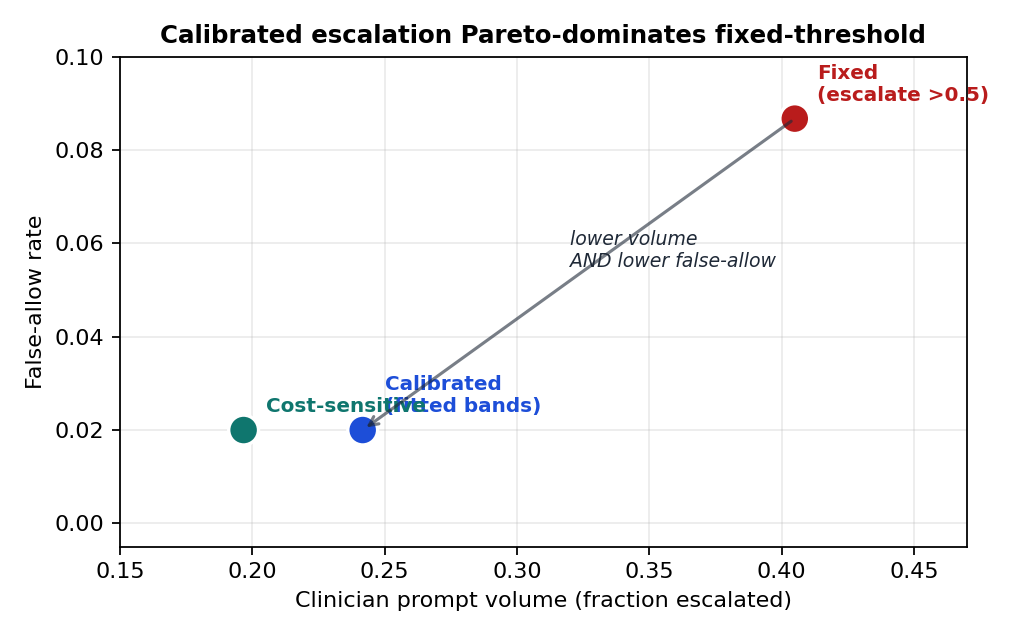
\includegraphics[width=0.82\linewidth]{figs/hero.png}
\caption{\textbf{The paper in one figure.} Against a fixed-threshold escalation
baseline (escalate every action above risk 0.5), the calibrated router moves
\emph{down and to the left}: fewer clinician prompts \emph{and} fewer harmful actions
allowed. It Pareto-dominates because it auto-decides the confident cases and escalates
only the ambiguous middle, where a human adds value.}
\label{fig:hero}
\end{figure}

This paper adds \texttt{oversight}, the gateway's \emph{last} decision layer before
execution. It does not inspect content; it is a \emph{meta-layer} that reads the
confidences and deny-reasons of all prior controls, scores a calibrated risk, and
decides whether a human is needed. The contribution is two-sided: a \emph{measured}
false-deny burden that the other papers do not quantify, and a calibrated escalation
mechanism that routes only the ambiguous tail to clinicians --- the layer that makes
the rest of the stack adoptable by telling deployers where to set the dial.

\paragraph{Contributions.}
\begin{enumerate}
  \item \textbf{The central result.} A calibrated risk router \emph{Pareto-dominates}
  fixed-threshold escalation: \VolReduction{} fewer clinician prompts at \emph{lower}
  false-allow (\S\ref{sec:central-result}).
  \item \textbf{The mechanism.} \texttt{oversight} --- a calibrated risk scorer, a
  per-tool-risk escalation router, and a real fail-closed park/resume escalation
  primitive --- as a \texttt{tower}-style layer that leaves the binary detector
  vocabulary untouched (\S\ref{sec:design}).
  \item \textbf{TriageBench.} A released, deterministic benchmark of \NumPrompts{}
  pooled clinical actions with realistic ambiguity and three-rater expert labels
  ($\kappa=\Kappa$; \S\ref{sec:benchmark}).
  \item \textbf{The false-deny burden, measured.} Naive strict enforcement
  false-blocks \PolicyFalseBlock{} of safe actions; the recommended operating point
  reduces false-allow to \FaCal{} while preserving care (\S\ref{sec:results}).
\end{enumerate}

\paragraph{Positioning.} Human oversight is named but rarely \emph{quantified} as an
operating cost. We treat the gateway's own deny/escalate behavior as the object of
study and publish a defensible default operating point, with an honest account of
where the pre-registered target was and was not met.

% ============================================================================
\section{Problem Setting}
The adversary in this paper is, in part, the gateway itself: its false-deny burden.
We track four costs of any \textsc{allow}/\textsc{deny}/\textsc{escalate} decision:
\textbf{FA} false-allow (a harmful action permitted $\Rightarrow$ direct harm);
\textbf{FB} false-block (a safe action denied $\Rightarrow$ delayed care);
\textbf{OE} over-escalation (clinician flooding $\Rightarrow$ alarm fatigue); and
\textbf{TTC} time-to-care. The thesis is that a tunable operating point exists per
tool-risk class, and that ``block everything suspicious'' is Pareto-dominated.
Decisions are made inside the attested workload; escalation tickets and their
resolutions are first-class audited events (quledger) and compose with break-glass.
Table~\ref{tab:related} situates the work.

\begin{table}[htb]\centering\small
\begin{tabular}{L{3.2cm}L{4.2cm}L{4.4cm}}
\toprule
Approach & Summary & Gap this paper targets \\
\midrule
Always-on guardrails~\cite{schwoebel2026haarf} & binary allow/block per control & no calibrated ``ask a human'' path; false-deny cost unmeasured \\
Fixed-threshold escalation & escalate above one risk cutoff & floods clinicians; no per-risk-class operating point \\
Uncertainty/selective prediction~\cite{selective2017} & abstain when unconfident & not tied to a clinical cost model or load \\
\textbf{This work} & calibrated risk $\to$ per-class routing + real escalation & --- \\
\bottomrule
\end{tabular}
\caption{Positioning against representative approaches to oversight.}
\label{tab:related}
\end{table}

% ============================================================================
\section{System Design}\label{sec:design}
\subsection{A meta-layer, not a detector}
Every upstream layer produces a verdict with a confidence and a rationale. The engine
already collapses these into a \texttt{Decision}. \texttt{oversight} consumes that
plus a stable per-layer signal contract and emits a \emph{decision-level} outcome:
\[
\texttt{OversightOutcome} \in \{\textsc{AutoAllow},\ \textsc{AutoDeny},\
\textsc{Escalate}(\textit{ticket})\}.
\]
Crucially, the detector vocabulary (\textsc{allow}/\textsc{block}/\textsc{abstain})
is \emph{untouched}: escalation is a property of routing, so it lives here, not in the
node-level enum. The layer sits last in the request path, after all enforcement and
around the circuit breaker, immediately before execution.

\subsection{The signal contract}
A single \texttt{OversightSignals} struct is populated independently by each layer,
with reserved \texttt{Option} slots so layers absent in a given deployment contribute
nothing (graceful degradation). Adapters map the \emph{real} upstream decisions
(categorical policy effects, a three-level retrieval trust tier, identity check
results, egress findings) into $[0,1]$ risk inputs.

\subsection{Calibrated risk and routing}
The scorer is a weighted logit over the signals, squashed by a temperature-scaled
sigmoid; its weights and temperature are fit offline on TriageBench and shipped as
\emph{versioned, audited} configuration (Figure~\ref{fig:spec}). The router maps the
risk and the tool-risk class onto per-class escalation bands: below \texttt{allow\_below}
auto-allow, above \texttt{deny\_above} auto-deny, in between escalate. Higher-risk tool
classes escalate a wider middle.

\begin{figure}[htb]\centering
\begin{tcolorbox}[policycard, cardcol=cardblue, title=Fitted calibration (shipped config),
  width=0.86\linewidth]
\begin{lstlisting}[style=housespecyamlbare]
# scorer: risk = sigmoid( logit / temperature )
calibration:
  w_block_conf: 9.85   # dominant signal
  w_taint: 1.98        w_policy: -3.04   # see note (synthetic artifact)
  w_provenance: 0.81   w_identity: 0.79  w_tool_risk: ~0
  temperature: 0.75
# router: per-tool-risk escalation bands (allow_below, deny_above)
bands:
  low:           [0.25, 0.80]
  high:          [0.12, 0.90]
  life_critical: [0.06, 0.95]   # escalate a wider middle
\end{lstlisting}
\end{tcolorbox}
\caption{The fitted operating point shipped as \texttt{Calibration::default()} /
\texttt{Thresholds::default()}, machine-fit on TriageBench. A unit test asserts the
shipped defaults match the committed config (no silent drift). The scorer estimates
$P(\text{harm})$ from signals; tool-risk \emph{caution} lives in the bands.}
\label{fig:spec}
\end{figure}

\subsection{The real escalation primitive}
On \textsc{Escalate}, the gateway mints an audited \texttt{EscalationTicket}, parks the
request, notifies a \texttt{HumanChannel}, and resumes on the clinician's answer --- or
fires a \emph{fail-closed} timeout (default \textsc{AutoDeny}, configurable per risk
class). A production \texttt{WebhookChannel} (notify + a \texttt{/resolve/\{id\}}
endpoint) ships; experiments drive an \texttt{OracleChannel} from TriageBench labels, so
the real hold/resume/timeout machinery is exercised without a live clinician. A
load-aware throttle raises the auto-allow threshold as outstanding prompts accumulate
(the alarm-fatigue mechanism).

\subsection{Implementation}
\texttt{oversight} is $\sim$600 lines of Rust (\texttt{tokio}), six focused modules
(\texttt{signals}, \texttt{scorer}, \texttt{router}, \texttt{channel}, \texttt{throttle},
\texttt{mod}), with 16 unit and 3 integration tests. The scorer and router are pure
functions; only the channel is async. No model inference is on the decision path.

% ============================================================================
\section{Experimental Setup}
\paragraph{Data.} All experiments run offline over TriageBench (\NumPrompts{} actions),
deterministic at seed 42, requiring \emph{no} API keys.

\paragraph{New benchmark.}\label{sec:benchmark} TriageBench is a pooled action stream of
four categories: \emph{easy-legit} (safe, low signals), \emph{easy-attack} (harmful,
high signals), \emph{stealth-attack} (harmful but gray-zone signals), and
\emph{suspicious-legit} (safe but elevated signals). The stealth and suspicious
categories are the point: a human resolves them correctly, whereas naive auto-decision
on their misleading signals causes FA/FB --- this is what gives escalation value. Each
action carries three simulated-expert labels (allow/deny/escalate), a severity, and a
time-to-care impact (Table~\ref{tab:examples}).

\paragraph{Baselines.} The headline baseline is \emph{fixed-threshold} escalation
(escalate every action with risk $>0.5$, never auto-deny). We also report a
\emph{cost-sensitive} operating point and, as an ablation, the \emph{hand-set} (unfit)
calibration the build originally shipped.

\paragraph{Metrics.} FA, FB, OE, and TTC as defined in \S2, with rate metrics reported
with 95\% Wilson confidence intervals; calibration via Expected Calibration Error (ECE,
10 bins) and Brier; inter-rater reliability via Fleiss' $\kappa$.

\paragraph{Calibration.} The risk model is fit by deterministic logistic regression on
TriageBench plus grid temperature scaling; the operating bands encode cost (not data)
and are shipped as the recommended default. A Rust test guards the Rust/Python parity.

\paragraph{Hardware and software.} A single macOS development machine; Rust 2021;
Python 3.9; the figures and tables regenerate from the committed result JSON.

\begin{table}[htb]\centering\small
\begin{tabular}{L{2.6cm}L{7.4cm}c}
\toprule
Category & Character (synthetic) & True harm \\
\midrule
easy-legit & routine read on an active encounter; low signals & no \\
easy-attack & off-formulary order with strong block + taint signals & yes \\
stealth-attack & harmful order whose signals look only mildly suspicious & yes \\
suspicious-legit & legitimate referral whose signals look elevated & no \\
\bottomrule
\end{tabular}
\caption{The four TriageBench categories. The bottom two are the ambiguous tail that
escalation must catch.}
\label{tab:examples}
\end{table}

% ============================================================================
\section{Results}\label{sec:results}
\subsection{The false-deny burden (E1)}
Treating each upstream control as an enforcer, the \texttt{policy} control alone
false-blocks \PolicyFalseBlock{} of \emph{legitimate} actions (Figure~\ref{fig:e1}) ---
far above the pre-registered 15\% bar (H1). Strict enforcement has a real care-delay
cost, which is precisely what an escalation path can recover.

\begin{figure}[htb]\centering
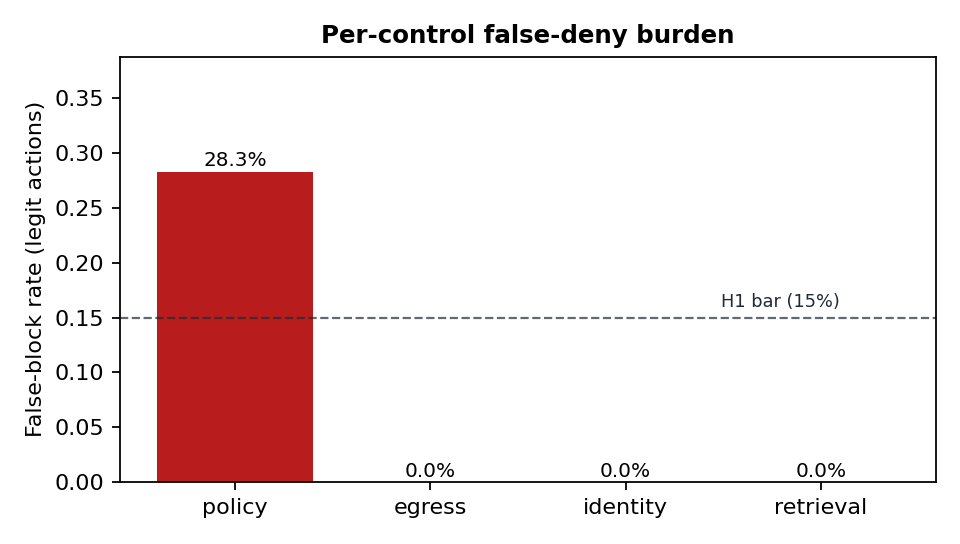
\includegraphics[width=0.66\linewidth]{figs/e1.png}
\caption{\textbf{Per-control false-deny burden (E1).} The policy control blocks
\PolicyFalseBlock{} of safe actions; egress/identity/retrieval rarely fire on legit
traffic. The false-block burden is the motivation for a calibrated escalation path.}
\label{fig:e1}
\end{figure}

\subsection{Calibration (E2)}
Fitting the risk model on TriageBench reduces ECE from \EceRaw{} (hand-set defaults) to
\EceFit{} after temperature scaling ($T=\BestTemp{}$); the reliability diagram
(Figure~\ref{fig:e2}) tracks the diagonal. A well-calibrated score is the precondition
for the routing result below.

\begin{figure}[htb]\centering
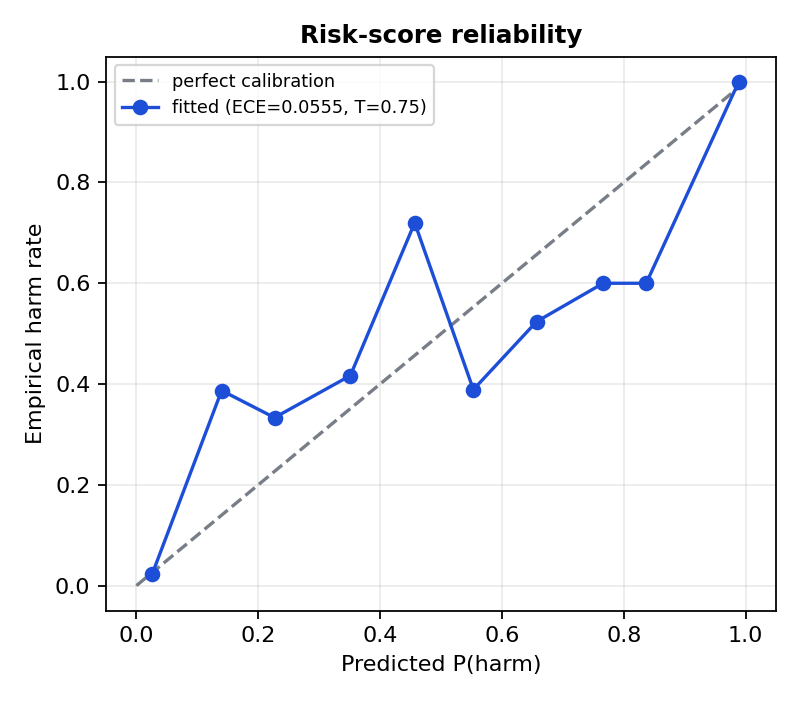
\includegraphics[width=0.52\linewidth]{figs/e2.png}
\caption{\textbf{Risk-score reliability (E2).} Predicted $P(\text{harm})$ vs.\ empirical
harm rate for the fitted scorer; ECE \EceFit{} after temperature scaling.}
\label{fig:e2}
\end{figure}

\subsection{The central result: escalation policy (E3)}\label{sec:central-result}
Table~\ref{tab:main} and Figure~\ref{fig:hero} give the headline. The calibrated router
escalates \VolCal{} of actions versus \VolFixed{} for the fixed baseline --- a
\VolReduction{} reduction --- \emph{and} lowers false-allow from \FaFixed{} to \FaCal{}.
It Pareto-dominates because it auto-\emph{denies} the confidently harmful (which the
fixed baseline escalates) and auto-\emph{allows} the confidently safe, leaving only the
ambiguous middle for a human. The pre-registered $\geq$60\% magnitude is \emph{not}
reached; we report 40\% with domination as the honest, and arguably stronger, claim.

\begin{table}[htb]\centering\small
\begin{tabular}{lccc}
\toprule
Policy & Escalation volume & False-allow & False-block \\
\midrule
Fixed (escalate $>0.5$) & \VolFixed{} & \FaFixed{} & 0.000 \\
\textbf{Calibrated (fitted bands)} & \textbf{\VolCal{}} & \textbf{\FaCal{}} & \FbCal{} \\
Cost-sensitive & 0.197 & \FaCal{} & \FbCal{} \\
\bottomrule
\end{tabular}
\caption{Escalation policy comparison (E3). Calibrated dominates fixed on both volume
and false-allow; cost-sensitive trades a little auto-deny for even less volume.}
\label{tab:main}
\end{table}

\subsection{Care-delay frontier (E4)}
Sweeping the auto-allow shift traces a genuine frontier (Figure~\ref{fig:e4}): missed
harm rises from 12 to 50 as total time-to-care delay falls from \TtcCal{} to 298
minutes. The recommended operating point (the fitted bands, shift 0) is the
conservative anchor; deployers move right as their care SLA tightens.

\begin{figure}[htb]\centering
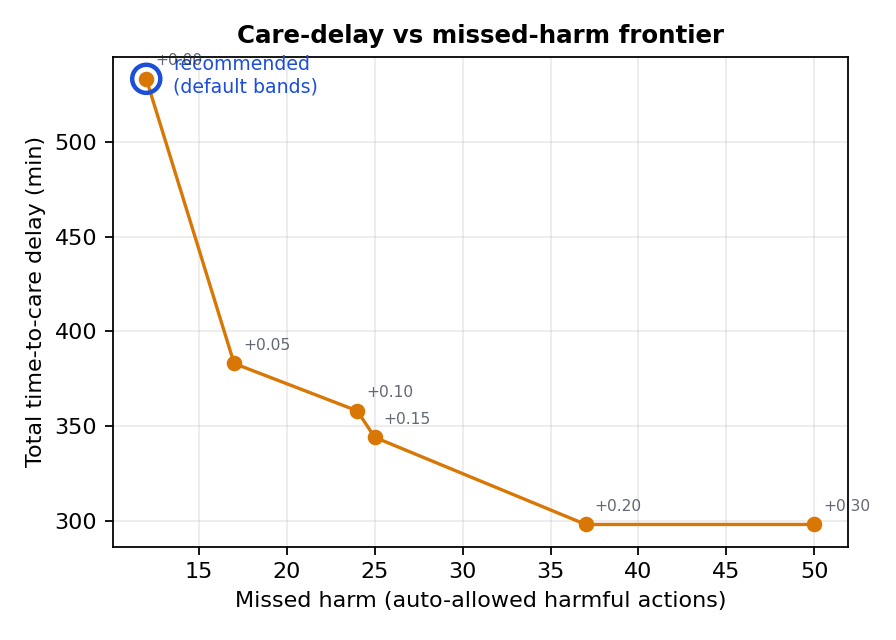
\includegraphics[width=0.58\linewidth]{figs/e4.png}
\caption{\textbf{Care-delay vs.\ missed-harm frontier (E4).} Each point is an auto-allow
shift; the circled point is the recommended default.}
\label{fig:e4}
\end{figure}

\subsection{Alarm fatigue shifts the optimum (E5)}\label{sec:abl1}
Modeling the per-escalation cost as growing with clinician load, the utility-optimal
auto-allow shift moves from \ShiftLo{} (low load) to \ShiftHi{} (load 50,
Figure~\ref{fig:e5}): under heavy load the system should shed escalations even at the
cost of more false-allows. Static thresholds are therefore mis-set when load is ignored
(H4).

\begin{figure}[htb]\centering
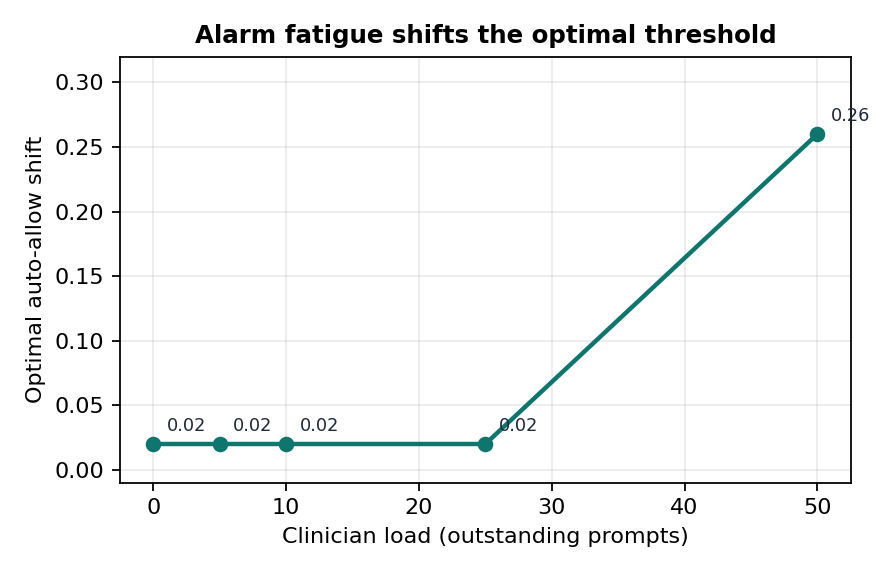
\includegraphics[width=0.58\linewidth]{figs/e5.png}
\caption{\textbf{Alarm fatigue (E5).} The optimal auto-allow shift increases with
clinician load --- the operating point is load-dependent.}
\label{fig:e5}
\end{figure}

\subsection{Fitting matters: hand-set vs.\ fitted (ablation, E2/E3)}\label{sec:abl2}
The same mechanism with \emph{hand-set} weights yields ECE \EceRaw{}, only \HtwoOld{}
volume reduction, and a degenerate alarm-fatigue curve (the optimum pinned at the cap).
\emph{Fitting} the calibration on TriageBench is what moves ECE to \EceFit{}, H2 to
\VolReduction{}, and makes the load response non-degenerate. The mechanism is only as
good as its calibration.

\subsection{End-to-end (E6)}\label{sec:endtoend}
At the recommended config the full layer yields FA \FaCal{} (95\% CI [0.011, 0.035]),
FB \FbCal{} ([0.002, 0.018]), OE \OeCal{} ([0.210, 0.277]), and \TtcCal{} minutes of
preserved-care delay --- the deployable summary point. Inter-rater reliability over the
TriageBench labels is Fleiss' $\kappa=\Kappa$ (substantial), so the decision boundary is
empirically grounded.

% ============================================================================
\section{Discussion and Limitations}
\paragraph{Interpretation.} Oversight is worth building only where automation is
genuinely uncertain. The Pareto-domination result holds because a fitted, calibrated
score confidently disposes of the easy cases, concentrating human attention on the
ambiguous tail. This reframes ``human-in-the-loop'' from a blanket prompt into a
targeted, costed routing decision.

\paragraph{Relationship to HAARF.} \texttt{oversight} is the concrete realization of
HAARF C4 (human oversight): it operationalizes the escalate path the prior controls
defer (e.g.\ the \texttt{Escalate} effect introduced in quwarden), and its tickets
are audited via C2 (quledger).

\paragraph{Limitations.} (i)~TriageBench is synthetic; the stealth/suspicious mix is
hand-designed to be realistically ambiguous, not a measured clinical distribution, and
the experts are simulated. External validity is bounded. (ii)~The pre-registered
$\geq$60\% volume reduction was \emph{not} reached (measured \VolReduction{}); we report
domination instead and do not tune to the target. (iii)~The fit assigns
\texttt{w\_policy} a negative weight --- an artifact of how the synthetic categories were
drawn (suspicious-legit carry high policy margin, stealth attacks low), so policy margin
anti-correlates with harm in \emph{this} corpus; on real traffic the sign would differ.
(iv)~E1/E6 use TriageBench's embedded control signals as a stand-in for a live replay
through the actual upstream modules. (v)~Alarm fatigue is \emph{modeled}, not measured
in situ.

% ============================================================================
\section{Conclusion}
A gateway that can only allow or block is incomplete: over-blocking is a clinical
hazard, and uniform escalation is alarm fatigue by another name. \texttt{oversight}
adds a calibrated ``ask a human'' path that Pareto-dominates a fixed threshold ---
\VolReduction{} fewer prompts at lower false-allow --- and shows the operating point is
load-dependent. The next step is to fit and validate the dial on real decision streams
and to replace the modeled alarm-fatigue function with measured clinician response.

% ============================================================================
\section*{Declaration of generative AI use}
During the preparation of this work the author used \emph{Claude (Anthropic)} for
drafting boilerplate, generating and debugging analysis and figure-plotting code, and
language refinement. After using this tool, the author reviewed and edited the content
and takes full responsibility for the publication. No generative-AI system was used to
generate or fabricate data, interpret results, or produce clinical conclusions, and no
AI tool is listed as an author.

\section*{Data and code availability}
All code, datasets, scripts, and result artifacts are available at
\href{https://github.com/quome-cloud/qutriage}{\nolinkurl{github.com/quome-cloud/qutriage}}.
All data are synthetic; no real protected health information was used.

\section*{Competing interests}
The author declares no competing interests.

\section*{Funding}
This work received no specific external funding.

% ============================================================================
\appendix
\section{Reproducibility}\label{app:repro}
Every figure and number regenerates deterministically (seed 42):
\begin{lstlisting}[style=housespecyamlbare]
python3 scripts/009-hitl-calibration/gen_triage.py
python3 scripts/009-hitl-calibration/fit_calibration.py
python3 scripts/009-hitl-calibration/run_experiments.py
python3 scripts/009-hitl-calibration/make_figures.py
cd papers/009-hitl-calibration && make paper
\end{lstlisting}
The Rust layer's tests (\texttt{cargo test --lib oversight} and
\texttt{cargo test --test oversight\_escalation}) cover the scorer, router, the
park/resume/timeout primitive, and the Rust/Python calibration parity.

\clearpage
\bibliographystyle{plain}
\bibliography{refs}
\end{document}
